%%%%%%%%%%%%%%%%%%%%%%%%%%%%%%%%%%%%%%%%%%%%%%%%%%%%%%%%%%%%%%%%%%%%%%%
%%%%%%%%%%%%%%%%%%%%%%%%%%%%%%%%%%%%%%%%%%%%%%%%%%%%%%%%%%%%%%%%%%%%%%%
%%%%%                                                                 %
%%%%%     <file_name>.tex                                             %
%%%%%                                                                 %
%%%%% Author:      <author>                                           %
%%%%% Created:     <date>                                             %
%%%%% Description: <description>                                      %
%%%%%                                                                 %
%%%%%%%%%%%%%%%%%%%%%%%%%%%%%%%%%%%%%%%%%%%%%%%%%%%%%%%%%%%%%%%%%%%%%%%
%%%%%%%%%%%%%%%%%%%%%%%%%%%%%%%%%%%%%%%%%%%%%%%%%%%%%%%%%%%%%%%%%%%%%%%

\chapter{Preliminaries / Background}
\section{Hero}
\section{Halide Language}
	\subsection { Programing model}
		Halide is a functionnal programming language,  embedded into C++ designed to write high performance image and array processing code \cite{Web:Halide}. This language uses a functionnal paradigm to describe the functionnalities of the processing pipeline. The code of the algorithm is separated from how it will be implemented on the  target (schedule). 


		Every pipeline is a function (\verb|Halide::Func| composed of other functions and expressions (\verb|Halide:expr|). These two objects  use special variables (\verb|Halide:Vars|) to describe the operation executed on the array. The code snippet~\ref{code:simple_pipeline} 
		describe a basic pipeline which compute the distance of each coordinate of a two-dimentionnal array from on position specified by the vector \verb|(center_x, center_y)|.


\lstset{basicstyle=\ttfamily\footnotesize,breaklines=true,tabsize=2}
\begin{lstlisting}[caption={Simple Pipeline Example}, captionpos=b, label={code:simple_pipeline}]
Halide::Var x, y;
Halide::Param center_x, center_y;
Halide::Expr offset = Halide::pow(x - center_x, 2) 
                      + Halide::pow(y - center_y, 2);

	gradient(x, y) = offset;
\end{lstlisting}
	This simple pipeline only has one stage, but it is possible to create multiple stage pipeline and transform it into a single stage inlined pipeline or keep it's multi stage structure, this operation will be done during the scheduling phase.

	After designing the  pipeline, we can define it's schedule via the different directive included in Halide. Halide implements all the basic scheduling option like parallelizing, unrolling the loops, splitting one loop into an inner and an outer loop... These options will be described in the section~\nameref{section:scheduling}. 

	In the example~\ref{code:simple_pipeline_schedule}, we can see how the scheduling works. All instructions are function of the pipeline object, and the final pipeline will implement these instructions. The example shows a simple schedule applied on our gradient, this schedule consists of parallelizing the execution over the x axis, and unrolling along the y axis.

	\begin{lstlisting}[caption={Simple Pipeline Example}, captionpos=b,label={code:simple_pipeline_schedule}];
	gradient.parallel(x);
	gradient.unroll(y, 10);
	\end{lstlisting}


	To execute the pipeline, Halide provides a large range of options, we can execute it directly using the \verb|.realize(x_max, y_max)| function, this is useful for debugging purpose, but most of the compile options are targeted at cross-compilation.
	
	As the initial goal of Halide was to target devices such as CPU, the library is capable of compiling the pipeline to a lot of different platform and output format. Halide support translation to C code, llvm assembly file, or already compiled object file specific to a given target(Cuda, Arm, Risc-V, MIPS, PowerPc...), and a given operating system( Linux, Mac, Windows, Android). The developer can also chose to compile the pipeline to a library to use in another application.

\subsection{Debugging Options}
	Halide has tools to debug the pipeline during it's compilation or when it is executed. First of all, the \verb|print()| and \verb|print_when()| functions can be called at any time in a pipeline and allow to print values of some variables. Another useful tool is the \verb|.trace_store()| function which prints the value every  functions evaluated in the pipeline. It is possible to get more informations during the compilation of the pipeline by setting the \verb|HL_DEBUG_CODEGEN| to 1, this will output the stages of the compilation and a pseudo code representation of the pipeline.
	Finally, variables and functions can have a label, which will be used by halide in it's internal representation, this function greatly reduce the debugging time of the schedules as Halide gives every variables a different name from the source code.


	\section {Basic Scheduling Options}
	\label{section:scheduling}

	Halide implement different scheduling instruction, and some of them just reshape the code in a different way. These scheduling instructions are useful to prepare the code for other instrutions (such as parallelization or vectorization), but also to  take advantage of memory locality.
\newcommand\EIW{.4\textwidth}
\newcommand\ECW{\textwidth - \EIW}
	\subsection{ Non Platform Specific Schedule}

	\subsubsection{Default Schedule}


\begin{figure}[h]
		\begin{minipage}[c]{\EIW}
			\centering
		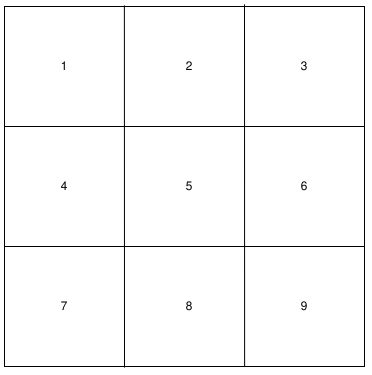
\includegraphics[width=\textwidth]{Images/BaseOrder.png}
		\end{minipage}
		\begin{minipage}[c]{\ECW}
			\centering
			\begin{lstlisting}[label={code:reorder}];
	for(int y = 0; y < 4; y++){
		for(int x = 0; x < 4; x++){
			do something ...
		}
	}
	
\end{lstlisting}
		\end{minipage}
	\caption{Base Schedule}
	\label{schedule:default}
\end{figure}



	If you don't specify any scheduling instructions, Halide will evaluate the pipeline in order. The first variable being the inner loop, and the last one the outer loop. In figure~\ref{schedule:default}, we can see the schedule in action, the image is processed in a row major fashion.

	\subsubsection{Reorder}


\begin{figure}[H]

		\begin{minipage}[c]{\EIW}
			\centering
		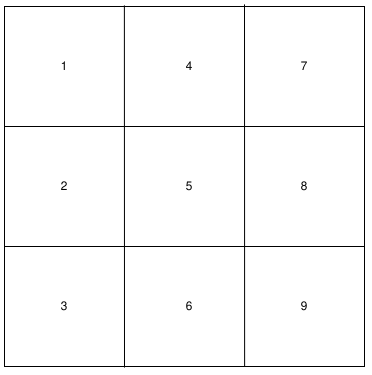
\includegraphics[width=\textwidth]{Images/Reorder.png}
		\end{minipage}
		\begin{minipage}[c]{\ECW}
			\centering
\begin{lstlisting}[label={code:reorder}];
	for(int x = 0; x < 4; x++){
		for(int y = 0; y < 4; y++){
			do something on
			(x,y)
		}
	}
\end{lstlisting}
		\end{minipage}
		\caption{Schedule: Reorder}
		\label{schedule:reorder}
\end{figure}



	The reorder instruction tells Halide how to traverse the domain space, using this instruction we can reorder the loops of the pipeline. In the exemple~\ref{schdule:reorder}, we changed the way the array is being processed from row major to column major.



	\subsubsection{Unroll}


\begin{figure}[H]
		\begin{minipage}[c]{\EIW}
			\centering
		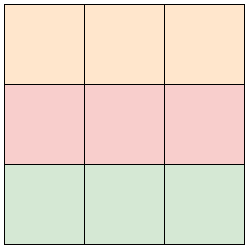
\includegraphics[width=\textwidth]{Images/Unroll.png}
		\end{minipage}
		\begin{minipage}[c]{\ECW}
			\centering
			\begin{lstlisting}[label={code:reorder}];
	for(int y = 0; y < 4; y++){
		do something on (0,y)
		do something on (1,y)
		do something on (2,y)
	}

\end{lstlisting}
		\end{minipage}
	\caption{Unroll Schedule}
	\label{schedule:unroll}
\end{figure}
	The Unroll schedule unrolls the code along one dimension. This instruction sometimes improve the code execution speed by removing the jumps at the end of each loop. This technique is often used by compilers to optimize the speed of the executable.

\subsubsection{Split}

\begin{figure}[H]

		\begin{minipage}[c]{\EIW}
			\centering
		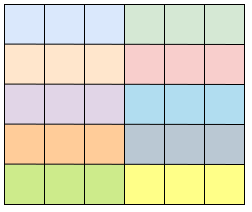
\includegraphics[width=\textwidth]{Images/Split.png}
		\end{minipage}
		\begin{minipage}[c]{\ECW}
			\centering
			\begin{lstlisting}[label={code:reorder}];
	for(int y = 0; y < 6; y++){
		for(int x_o = 0; x_o < 3; x_o++){
			for(int x_i = 0; x_i < 4; x_i++){

				do something on
				(x_o * 3 + x_i, y)
			}
		}
	}
\end{lstlisting}
		\end{minipage}
		\caption{Schedule Split}
\end{figure}

	This schedule replaces one loop over a dimension by two loops, an inner loop and an outer loop. This schedule is useful to cut the array in smaller pieces that will be computed in parallel or using \gls{simd} instructions.

\subsubsection{Tile}


\begin{figure}[H]

		\begin{minipage}[c]{\EIW}
			\centering
		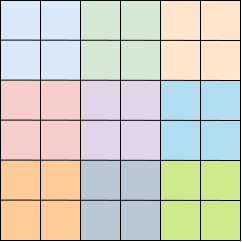
\includegraphics[width=\textwidth]{Images/Tile.png}
		\end{minipage}
		\begin{minipage}[c]{\ECW}
			\centering
			\begin{lstlisting}[label={code:reorder}];
	for(int y_o = 0; y_o < 6; y_o++){
		for(int x_o = 0; x_o < 3; x_o++){
			for(int y_i = 0; y_i < 2; y_i++){
				for(int x_i = 0; x_i < 2; x_i++){
					do something on
					(x_o * 2 + x_i, y_o * 2 + y_i)
				}
			}
		}
	}
\end{lstlisting}
		\end{minipage}
		\caption{Schedule Tile}
\end{figure}
	The Tile schedule is similar to the Split schedule, but along two dimensions. It creates multiples smaller rectangles which can be processed independantly.

	\subsection{Platform Specific Schedules}
\subsubsection{Parallel}
\begin{figure}[H]

		\begin{minipage}[c]{\EIW}
			\centering
		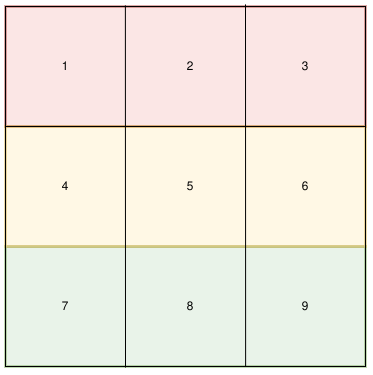
\includegraphics[width=\textwidth]{Images/Parallel.png}
		\end{minipage}
		\begin{minipage}[c]{\ECW}
			\centering
			\begin{lstlisting}[label={code:reorder}];
	# Core 0: y = 0
	for(int x = 0; x < 4; x++){
		do something on (x,0)
	}

	# Core 1: y = 1
	for(int x = 0; x < 4; x++){
		do something on (x,1)
	}

	# Core 2: y = 2
	for(int x = 0; x < 4; x++){
		do something on (x,2)
	}
	}
\end{lstlisting}
		\end{minipage}
		\caption{Schedule Parallel}
		\label{schedule:parallel}
\end{figure}

The parallel schedule allows the pipeline to be distributed to all the available cores. Halide will create for task for each value the variable can take, and these tasks will be executed with the \verb|halide_do_par_for| function. This function has been overwritten on hero to execute on the \gls{pulp} cluster. In the example~\ref{schedule:parallel}, the code is distributed on three cores, each of them execute a single loop along the y axis.

	\subsubsection{Vectorize}
	The goal of this schedule is to setup the code so to make use of the \gls{simd} instructions of the \gls{cpu}. Currently, llvm doesn't support the vector extension  implemented in the pulp cluster, but the generated code will take advantages of all the registers available to compute the output values, ans try to compute multiple values at the same time.



	\subsection { Porting Halide to new Platforms}
		First of all, to compile to a specific platform, we need a build of llvm which support the desired architecture.
		Then we can look in the pipeline header file to list all the vital functions for our pipeline. We can also use the error message when linking the pipeline to determine which functions we need to implement on the target platform. 
		Currently only the memory allocation functions, the print functions and the task distribution functions are implemented, and they are enough to  test basic pipelines such as matrix multiplications or light image modifications.
	After the implementation we can work on the compilation workflow for hero.

\section{Compilation Workflow}
	Every application has at least two source files, one C++ file which will generate the object file of the pipeline, the main application. 
	Currently, we can only compile the application to the hardware simulator.
	The compilation has two phases, during the first one, we compile the Halide application using llvm and run it on the host platform, this application will then generate an risc-V object file and a header.
	Then we compile the hero application using the already available Makefile, we include the header in the main application and the object file to the sources during the linking command.

		
\section{The full hero platform}
	The hardware platform has a more complex compiling process, currently the code is distributed to the \gls{pulp} thanks to OpenMp. The compilation first generate the llvm representation of the  code, then assign space on the device via \verb|hc-omp-space|, and also \verb|clang-offload-bundler| to distribute generate the llvm assembly code for the right platform. Finally the  program uses clang to compile the application, thanks to the special hero target, clang links every function correctly and then embed the riscV code inside the ARM application.

%%% Local Variables: 
%%% mode: latex
%%% TeX-master: "../report_template"
%%% End: 
